\documentclass[11pt,a4paper]{article}
\usepackage[margin=22mm,footskip=11mm]{geometry}
\usepackage{graphicx,booktabs,amsmath,xcolor,fancyhdr}
\usepackage{xepersian}
\settextfont[Path=assets/fonts/]{Vazirmatn-Regular.ttf}
\definecolor{navy}{HTML}{173B4C}
\definecolor{teal}{HTML}{256B83}
\pagestyle{fancy}
\fancyhf{}
\fancyhead[R]{\textcolor{teal}{پروژهٔ درس آمار}}
\fancyhead[L]{\textcolor{teal}{\lr{TCGA-BRCA}}}
\fancyfoot[C]{\thepage}
\setlength{\headheight}{16pt}
\setlength{\parskip}{.65em}
\setlength{\parindent}{0pt}
\newcommand{\reporttitle}[1]{\par\vspace{.7em}{\Large\textcolor{navy}{#1}}\par\vspace{.4em}}
\newcommand{\num}[1]{\lr{#1}}
\newcommand{\pct}[1]{\lr{#1\%}}
\begin{document}

{\LARGE\textcolor{navy}{فاز دوم پروژهٔ آمار}}\par
{\large احتمال و توزیع‌های احتمالی در داده‌های سرطان پستان}\par
\textcolor{teal}{پاییز ۱۴۰۵ | مسیر ب | داده‌های بالینی و بیان ژن}

\reporttitle{۱. سؤال و فضای نمونه}
آیا بین قرارگرفتن بیان \lr{MKI67} بالاتر از میانه و قرارگرفتن بیمار در مرحلهٔ پاتولوژیک پیشرفته تفاوت تجربی دیده می‌شود؟ شکل توزیع بیان ژن چیست و کوواریانس آن با سن هنگام تشخیص چه علامتی دارد؟

واحد تحلیل بیمار است. داده از جدول پردازش‌شدهٔ فاز اول و نسخهٔ \lr{@@release@@} گرفته شده است. برای هر بیمار همان تشخیص اصلی یکتا و همان نمونهٔ تومور اولیهٔ منتخب فاز اول را نگه داشتیم. اگر چند فایل بیان ژن موجود بود، شناسهٔ نمونه، شناسهٔ بخش نمونه و سپس شناسهٔ فایل به ترتیب لغت‌نامه‌ای ملاک انتخاب بودند. یکتایی شناسهٔ بیمار و شناسهٔ مورد قبل از محاسبه کنترل شد.

\begin{center}
\begin{tabular}{rcc}
\toprule
تحلیل & تعداد بیمار & شرط ورود \\
\midrule
دادهٔ پیوندخورده & @@cohort_n@@ & اطلاعات بالینی و نمونهٔ تومور اولیه \\
توزیع بیان ژن & @@marker_n@@ & مقدار معتبر ژن \\
احتمال مرحله و بیان & @@event_n@@ & مقدار معتبر ژن و مرحله \\
کوواریانس سن و بیان & @@pair_n@@ & مقدار معتبر ژن و سن \\
\bottomrule
\end{tabular}
\end{center}

در جدول پیوندخورده، مرحله برای @@missing_stage@@ بیمار و سن برای @@missing_age@@ بیمار گمشده است. تعداد مقادیر گمشدهٔ \lr{MKI67} برابر @@missing_marker@@ است. هر تحلیل از ردیف‌هایی استفاده می‌کند که متغیرهای همان تحلیل را دارند.

\reporttitle{۲. رویدادها و متغیرهای تصادفی}
\(X=\log_2(\text{FPKM-UQ}+1)\) بیان ژن و \(Y\) سن هنگام تشخیص بر حسب سال است. رویداد \(A\) یعنی مرحلهٔ \lr{III} یا \lr{IV} و مکمل آن در جدول معتبر یعنی مرحلهٔ \lr{I} یا \lr{II}. رویداد \(B\) یعنی \(X\) به‌طور اکید بالاتر از میانهٔ بیان در تمام بیماران دارای دادهٔ ژن باشد. آستانهٔ \num{@@median@@} بدون استفاده از مرحله یا سن و پیش از ساخت جدول احتمال تعیین شد. تساوی با آستانه در گروه پایین قرار می‌گیرد؛ تعداد تساوی‌ها @@median_ties@@ است. این آستانه صرفاً یک قاعدهٔ آموزشی برای گروه‌بندی بیان RNA است.

\newpage
\reporttitle{۳. احتمال تجربی و استقلال}
فضای نمونهٔ تجربی برای این بخش شامل @@event_n@@ بیمار با مرحله و مقدار بیان معلوم است. همهٔ بیماران در این فضا وزن برابر دارند. در هر خانه تعداد و احتمال مشترک نسبت به کل جدول آمده‌اند. جمع ردیف‌ها و ستون‌ها احتمال حاشیه‌ای را می‌دهد.

\begin{center}
\begin{tabular}{rccc}
\toprule
مرحله & بیان تا میانه & بیان بالاتر از میانه & جمع \\
\midrule
\lr{I–II} & \num{@@Count00@@ (@@Joint00@@\%)} & \num{@@Count01@@ (@@Joint01@@\%)} & @@early_total@@ \\
\lr{III–IV} & \num{@@Count10@@ (@@Joint10@@\%)} & \num{@@Count11@@ (@@Joint11@@\%)} & @@advanced_total@@ \\
جمع & @@low_total@@ & @@high_total@@ & @@event_n@@ \\
\bottomrule
\end{tabular}
\end{center}

\begin{latin}
\begin{align*}
\widehat P(A) &= @@advanced_total@@/@@event_n@@ = @@p_advanced@@, &
\widehat P(B) &= @@high_total@@/@@event_n@@ = @@p_high@@,\\
\widehat P(A\cap B) &= @@Count11@@/@@event_n@@ = @@p_both@@, &
\widehat P(A)\widehat P(B) &= @@independent_joint@@,\\
\widehat P(A\mid B) &= @@Count11@@/@@high_total@@ = @@p_stage_given_high@@, &
\widehat P(A\mid B^c) &= @@Count10@@/@@low_total@@ = @@p_stage_given_low@@.
\end{align*}
\end{latin}

احتمال تجربی مرحلهٔ پیشرفته در گروه بالاتر از میانه \pct{@@pct_p_stage_given_high@@} و در گروه دیگر \pct{@@pct_p_stage_given_low@@} است. اختلاف گروه بالاتر منهای گروه پایین \num{@@pct_stage_given_high_minus_low@@} واحد درصد است. احتمال مشترک هم تنها \num{@@pct_joint_gap@@} واحد درصد با حاصل‌ضرب حاشیه‌ها فاصلهٔ علامت‌دار دارد. جدول برای این دو رویداد تقریباً با الگوی استقلال هم‌خوان است. این مقایسه توصیفی و محدود به گروه‌بندی انتخاب‌شده است.

\reporttitle{۴. وارون‌کردن شرط با قضیهٔ بیز}
وقتی فقط مرحله را می‌دانیم، احتمال بیان بالای میانه در گروه پیشرفته \pct{@@pct_p_high_given_stage@@} و در گروه زودرس \pct{@@pct_p_high_given_early@@} است. برای پرسش معکوس، یعنی احتمال مرحلهٔ پیشرفته پس از دیدن بیان بالاتر از میانه، محاسبهٔ بیز با تقسیم مستقیم جدول برابر است.
\[
\widehat P(A\mid B)=\frac{\widehat P(B\mid A)\widehat P(A)}{\widehat P(B)}
=\frac{(@@Count11@@/@@advanced_total@@)(@@advanced_total@@/@@event_n@@)}{@@high_total@@/@@event_n@@}
=@@bayes@@.
\]
\begin{center}
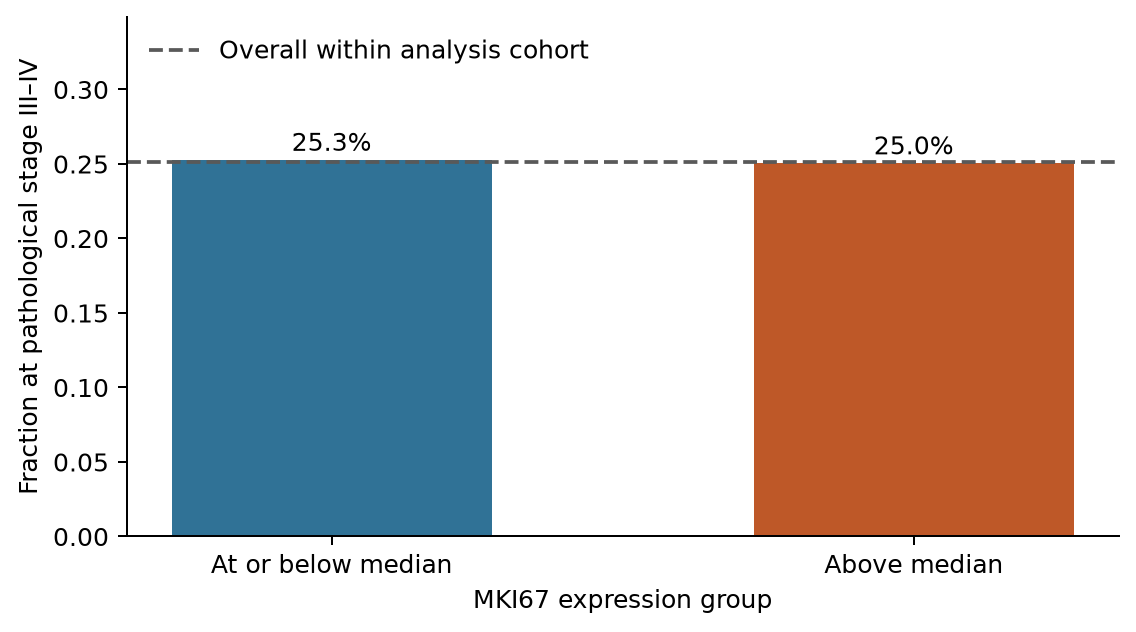
\includegraphics[width=.69\linewidth]{figures/phase2/01_conditional_probability.png}
\end{center}

\newpage
\reporttitle{۵. شمارش بیماران با بیان بالا}
متغیر تصادفی \(K\) تعداد بیماران دارای \(B\) در @@n_draws@@ برداشت یکنواخت از جدول احتمال است. در برداشت با جایگذاری، هر برداشت مستقل است و احتمال موفقیت ثابت \(p=@@high_total@@/@@event_n@@\) دارد. بنابراین
\[
P(K=k)=\binom{@@n_draws@@}{k}p^k(1-p)^{@@n_draws@@-k}.
\]
میانگین مدل \num{@@binomial_mean@@} بیمار و واریانس آن \num{@@binomial_var@@} بیمار مربع است. برای برداشت بدون جایگذاری، انتخاب قبلی تعداد افراد باقی‌مانده را تغییر می‌دهد و توزیع دقیق فوق‌هندسی با \(N=@@event_n@@\) و \(M=@@high_total@@\) است.
\[
P(K=k)=\frac{\binom{M}{k}\binom{N-M}{@@n_draws@@-k}}{\binom{N}{@@n_draws@@}}.
\]
میانگین ثابت می‌ماند، اما واریانس به \num{@@hypergeometric_var@@} کاهش می‌یابد. نصف مجموع اختلاف قدرمطلق احتمال‌ها در دو توزیع \num{@@pmf_total_variation@@} است. کسر نمونه‌گیری حدود دو درصد است و نمودار نشان می‌دهد در این اندازهٔ نمونه تقریب دوجمله‌ای نزدیک است. این مقایسه بر پایهٔ طرح فرضی برداشت از همین جدول انجام شده است.

\begin{center}
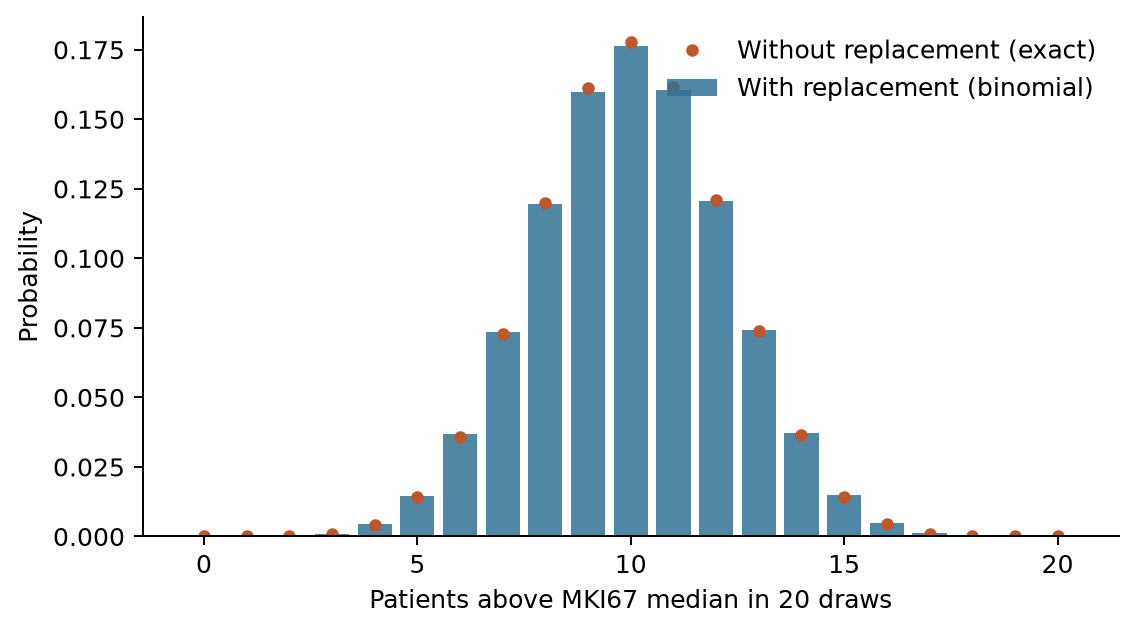
\includegraphics[width=.88\linewidth]{figures/phase2/02_count_model.png}
\end{center}

برای یک بیمار با شانس انتخاب برابر، شاخص \(1_B\) توزیع برنولی دارد. امید آن \(p\) و واریانس آن \(p(1-p)\) است. در مدل با جایگذاری، \(K\) مجموع @@n_draws@@ شاخص مستقل است؛ به همین دلیل واریانس‌های آن‌ها جمع می‌شوند. نمونه‌های متعدد تومور یک بیمار حق انتخاب آن بیمار را افزایش نمی‌دهند.

\newpage
\reporttitle{۶. توزیع بیان \lr{MKI67} و تقریب نرمال}
میانگین تجربی \num{@@mean@@} و واریانس تجربی \num{@@variance_empirical@@} روی مقیاس لگاریتمی به دست آمدند. میانگین مقدار مورد انتظار بیان یک بیمار منتخب از جدول و واریانس متوسط مربع فاصله از آن است. برای توصیف همین توزیع تجربی بر \(n\) تقسیم می‌کنیم. واریانس با مخرج \(n-1\) برابر \num{@@variance_sample@@} است.

میانه \num{@@median@@}، چارک اول \num{@@q1@@}، چارک سوم \num{@@q3@@} و دامنه از \num{@@min@@} تا \num{@@max@@} است. طبق قاعدهٔ فاصلهٔ \(1.5\,\mathrm{IQR}\) از چارک‌ها، @@lower_outliers@@ مقدار در پایین و @@upper_outliers@@ مقدار در بالا پرچم می‌خورند. مقدار پرچم‌خورده در محاسبه حفظ شده است. چولگی تجربی \num{@@skewness@@} است.

\begin{center}
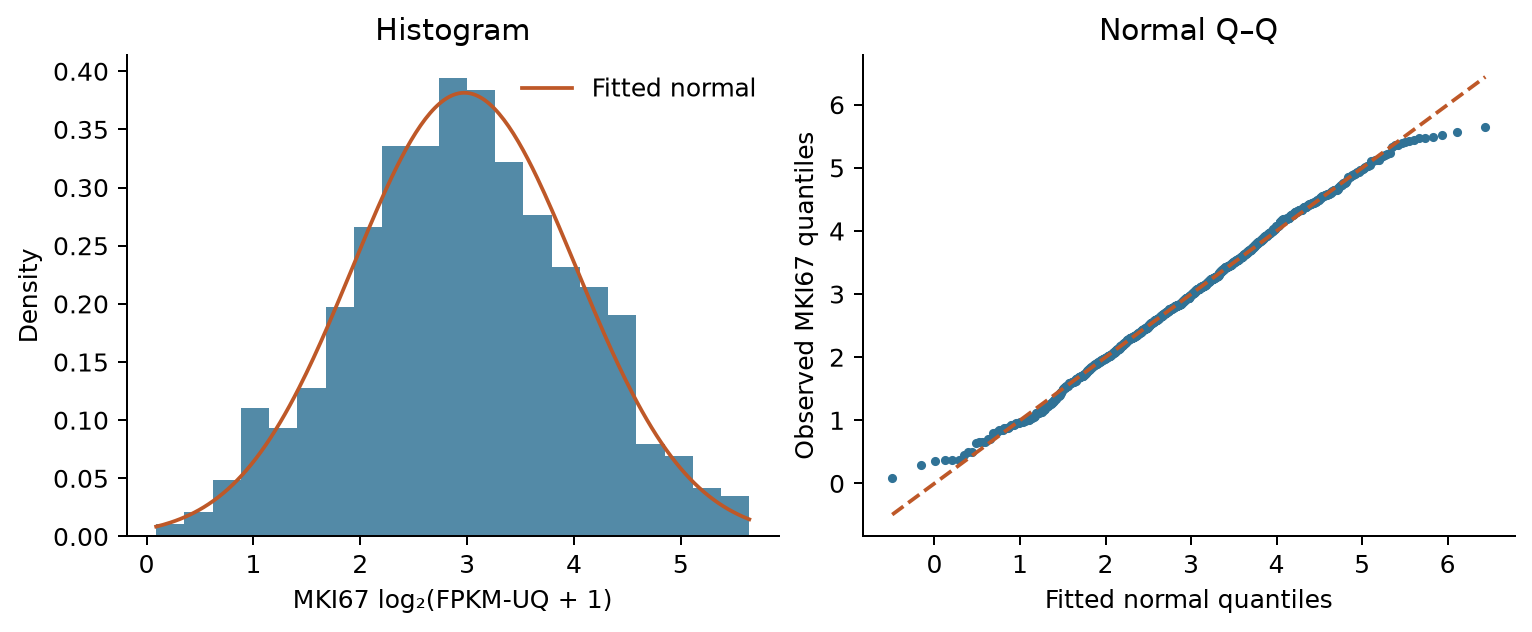
\includegraphics[width=\linewidth]{figures/phase2/03_mki67_distribution.png}
\end{center}

هیستوگرام با چگالی نرمال برازش‌شده بر میانگین و انحراف معیار تجربی مقایسه شده است. در نمودار \lr{Q–Q}، محور افقی چندک‌های همان نرمال و محور عمودی چندک‌های مشاهده‌شدهٔ ژن را نشان می‌دهد. نزدیکی بخش میانی به خط قطری و انحراف دو سر نمودار به تفکیک مرکز و دنباله‌ها کمک می‌کند. @@normal_direction@@ نرمال برازش‌شده برای مقادیر منفی احتمال \pct{@@pct_normal_below_zero@@} می‌گذارد، در حالی که مقدار تبدیل‌شدهٔ بیان ژن نامنفی است.

\newpage
\reporttitle{۷. رابطهٔ سن هنگام تشخیص با بیان ژن}
برای @@pair_n@@ بیمار دارای هر دو مقدار، سن و بیان ژن بر حسب مقیاس‌های بخش دوم به‌صورت زوجی وارد محاسبه شدند.
\[
\widehat{\operatorname{Cov}}(Y,X)
=\frac{1}{n}\sum_{i=1}^n(Y_i-\bar Y)(X_i-\bar X)
=@@covariance_empirical@@.
\]
واحد کوواریانس سال ضرب در واحد بیان روی مقیاس لگاریتمی است. کوواریانس با مخرج \(n-1\) برابر \num{@@covariance_sample@@} به دست می‌آید. علامت @@covariance_direction@@ یعنی حاصل‌ضرب انحراف‌های زوج‌ها در مجموع @@covariance_direction@@ است. در نمودار پراکندگی هر نقطه یک بیمار است و خط‌های نقطه‌چین میانگین دو متغیر را نشان می‌دهند. پراکندگی در سن‌های مشابه قابل توجه است و مقدار کوواریانس به واحدهای اندازه‌گیری وابسته است.

\begin{center}
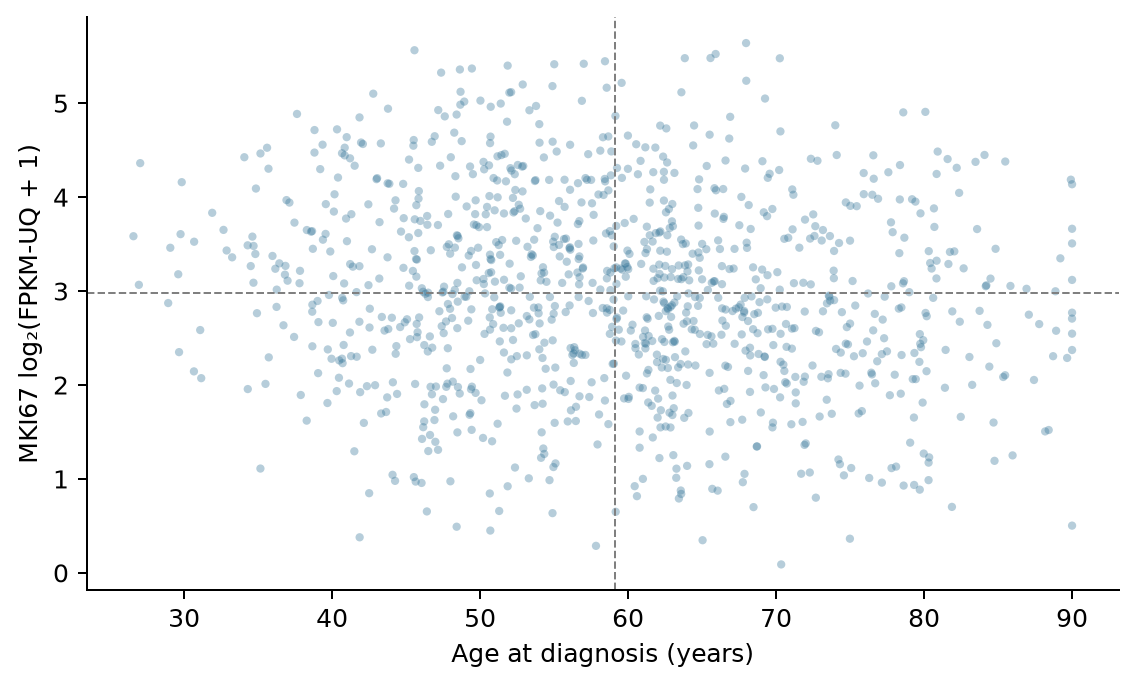
\includegraphics[width=.86\linewidth]{figures/phase2/04_age_mki67.png}
\end{center}

\reporttitle{۸. دامنهٔ تفسیر و بازتولید}
این احتمال‌ها به گروه بیماران واردشده در جدول مربوط‌اند. گمشدگی مرحله و سن می‌تواند ترکیب نمونهٔ هر محاسبه را عوض کند. مرحله‌بندی دودویی و نصف‌کردن مقیاس پیوسته نیز بخشی از اطلاعات را کنار می‌گذارد. فاز حاضر توصیفی است و اندازهٔ اثر جمعیتی، تشخیص بالینی یا اثر علّی را برآورد نمی‌کند.

\lr{data/README.md} منشأ داده و قواعد پیوند را مستند می‌کند. محاسبات با \lr{src/analyze\_phase2.py} و گزارش با \lr{src/build\_phase2\_report.py} بازتولید می‌شوند. اثر انگشت \lr{SHA-256} جدول ورودی در \lr{reports/phase2/results.json} ثبت شده است.

{\small کد، محاسبات و پیش‌نویس گزارش با کمک دستیار هوش مصنوعی تهیه شده‌اند. بازبینی علمی و دفاع از تصمیم‌ها بر عهدهٔ دانشجو است.}
\end{document}
